% chapters/glitch.tex
%
% Copyright 2023 Alexander Lyttle.
%
% This work may be distributed and/or modified under the conditions of the
% LaTeX Project Public License (LPPL) version 1.3 or later.
%
% The latest version of this license is in
% https://www.latex-project.org/lppl.txt and version 1.3 or later is part of
% all distributions of LaTeX version 2005/12/01 or later.
%
%
\chapter[Acoustic Glitches in Solar-Like Oscillators]{Acoustic Glitches in Solar-Like Oscillators as a Signature of Helium Abundance}\label{chap:glitch}

\textit{In this chapter, I explore an asteroseismic signature of helium which could provide observables to add to the hierarchical model from Chapter \ref{chap:hmd}. I introduce the concept of an acoustic glitch in the structure of a star producing a measurable signal in its observable oscillation modes. In Section \ref{sec:1d-glitch}, I start with a simple one-dimensional example of a glitch. Then, I review the theory of glitch signatures due to helium ionisation and the base of the convective zone in Section \ref{sec:glitch-star}.}

\section{Introduction}
% \epigraph{\singlespacing``Ideals are like stars: you will not succeed in touching them with your hands, but like the seafaring man on the ocean desert of waters, you choose them as your guides, and following them, you reach your destiny.''}{\emph{Carl Schurz}}

% So far in this thesis, we have shown that a hierarchical Bayesian model can be used to infer the helium abundance distribution in a stellar population. We also found how this improves the inference of fundamental stellar parameters. However, there is limited information about helium abundance in the stellar observables used (e.g. \(L, \teff, \Delta\nu\)).

An acoustic glitch is a rapid variation of the sound speed inside a medium. The presence of a glitch induces a periodic signature in consecutive p mode frequencies. Acoustic glitches in Sun-like stars arise from sharp variations in their structure, such as the base of the convection zone (BCZ) and the first and second ionisation of helium (He\,\textsc{i} and He\,\textsc{ii}). There have been several attempts to measure this effect in the Sun and other stars over the past few decades.

Early work identified glitches in solar p modes by analysing their second differences, \(\Delta_2\nu_{nl} \equiv \nu_{n-1\,l} - 2\nu_{nl} + \nu_{n+1\,l}\). Second and higher-order differences remove some slowly varying components of the mode frequencies and amplify faster varying components. Assuming a sharp localised discontinuity in sound speed at He\,\textsc{ii} ionisation and the BCZ, \citet{Basu.Antia.ea1994,Basu1997} modelled glitch signatures in the Sun to constrain the extent of convective overshoot at the BCZ. \citet{Monteiro.Thompson1998} further developed a model of the He\,\textsc{ii} ionisation glitch signature by accounting for its finite width in the star, later applying it to study the helium ionisation zone of the Sun \citep{Monteiro.Thompson2005}. Around the same time, \citet{Basu.Mazumdar.ea2004} showed that the amplitude of the He\,\textsc{ii} glitch signature correlated with the fractional helium abundance (\(Y\)) near the surface of Sun-like stars. A few years later, \citet{Houdek.Gough2007} proposed a closer physical approximation of the He\,\textsc{ii} glitch. They derived the glitch signature which was later used in several studies of solar-like oscillators.

Since helium ionises below the stellar atmosphere for cool stars (\(\teff \sim \SI{e5}{\kelvin}\)), asteroseismology was able to probe helium abundance where spectroscopy could not. Glitches could be further studied in stars other than the Sun with the advent of space-based missions. \citet{Miglio.Montalban.ea2010,Mazumdar.Michel.ea2012} were among the first to measure glitch signatures in other stars after \emph{CoRoT} provided evidence of solar-like oscillations in red giants. Then, studies of glitches in main sequence stars observed by \emph{Kepler} compared fitting to the modes frequencies directly with using second differences \citep{Mazumdar.Monteiro.ea2012,Mazumdar.Monteiro.ea2014,Verma.Raodeo.ea2017}. More recently, \citet{Verma.Raodeo.ea2019} used measurements of the glitch to estimate the helium abundance for the LEGACY sample of stars \citet{Lund.SilvaAguirre.ea2017}.

The reason that acoustic glitches cause a periodic signal in the mode frequencies is not obvious. Hence, we go through a simple, one-dimensional example in Section \ref{sec:1d-glitch}. Then, in Section \ref{sec:glitch-star}, we demonstrate how glitches in stellar structure due to helium ionisation and the BCZ affect the mode frequencies of solar-like oscillators. Starting with the variational principle \citep{Chandrasekhar1964}, we show how to get to the He\,\textsc{ii} glitch signature formula from \citet{Houdek.Gough2007}.

\section[1D Glitch Example]{A One-Dimensional Example of a Glitch}\label{sec:1d-glitch}

\newcommand*{\glitch}{\ensuremath{{\mathrm{g}}}}

A rapid variation in the structure of a medium induces a periodic perturbation (\(\delta\omega\)) to the eigenfrequencies. To demonstrate this, we will explore a simple one-dimensional example \citep[similar to that of][]{Verner2005}. Consider a medium bound from \(x=0\) to \(x=L\) in which pressure waves can propagate at constant speed, \(c\). The longitudinal displacement of the wave (\(\xi\)) obeys the wave equation,
%
\begin{equation}
    \frac{\partial^2\xi(x, t)}{\partial t^2} = c^2 \frac{\partial^2\xi(x, t)}{\partial x^2},
\end{equation}
%
at a given position (\(x\)) and time (\(t\)). We may write a general solution to the wave as a sum of right- and left-travelling waves. In terms of the angular frequency (\(\omega\)), wave number (\(k\)), and complex coefficients \((A, B)\),
%
\begin{equation}
    \xi(x, t) = A \ee^{i (\omega t - k x)} + B \ee^{i (\omega t + k x)},
\end{equation}
%
where \(\omega\) and \(k\) satisfy \(\omega = c k\). Solving for the boundary condition, \(\xi(0, t) = 0\), we find \(B = - A\). Substituting Euler's formula, \(A = (r/2) \ee^{i\phi}\), we can represent the physical component of the wave by its real solution,
%
\begin{equation}
    \real\left[\xi(x, t)\right] = r \sin k x \sin(\omega t + \phi),
\end{equation}
%
where \(r\) and \(\phi\) are the amplitude and temporal phase respectively. Solutions for \(\omega\) which satisfy \(\xi(L, t)=0\) may then be found,
%
\begin{equation}
    \omega_n = c \frac{n \pi}{L}, \label{eq:omega-n}
\end{equation}
%
where \(n\) is a non-zero integer (the \(n=0\) solution would give \(\xi=0\) everywhere).

\begin{figure}[!tb]
    \centering
    % 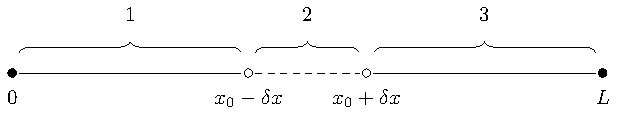
\includegraphics{figures/glitch-1d-example-diagram.pdf}
    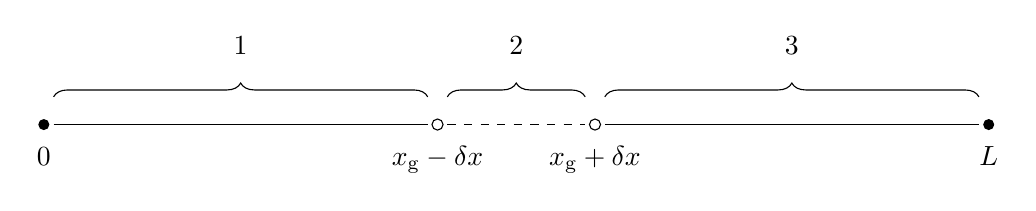
\begin{tikzpicture}
  \def\labelshift{(0, -0.4)}%
  \def\regionshift{(0, 1)}%
  \node[label={[anchor=base,shift=\labelshift]below:0}] (A) at (0, 0) {};
  \node[label={[anchor=base,shift=\labelshift]below:$x_{\mathrm{g}}-\delta x$}] (B) at (5, 0) {};
  \node[label={[anchor=base,shift=\labelshift]below:$x_{\mathrm{g}}+\delta x$}] (C) at (7, 0) {};
  \node[label={[anchor=base,shift=\labelshift]below:$L$}] (D) at (12, 0) {};

  \fill (A) circle (2pt) (D) circle (2pt);
  \draw (B) circle (2pt) (C) circle (2pt);
  \draw (A) -- (B) (C) -- (D);
  \draw[dashed] (B) -- (C);

  \draw[decorate,decoration={brace,amplitude=5pt,raise=10pt}] (A) -- (B) node[midway,shift=\regionshift]{1};
  \draw[decorate,decoration={brace,amplitude=5pt,raise=10pt}] (B) -- (C) node[midway,shift=\regionshift]{2};
  \draw[decorate,decoration={brace,amplitude=5pt,raise=10pt}] (C) -- (D) node[midway,shift=\regionshift]{3};
\end{tikzpicture}

    \caption[A diagram showing a one-dimensional medium with a small structural perturbation.]{A diagram showing a one-dimensional medium split into three regions. 1: Fixed at \(x=0\) with a constant speed of sound \(c\); 2: A small structural perturbation centred at \(x=x_\glitch\) with width \(2\delta x\) and constant speed of sound \(c + \delta c\); 3: Fixed at \(x=L\) with a constant speed of sound \(c\).}
    \label{fig:1d-diagram}
\end{figure}

Now, let us suppose there is a small structural perturbation (or glitch) in the medium at position \(x_\glitch\) with half-width \(\delta x\). Figure \ref{fig:1d-diagram} shows this system divided into 3 regions, with region 2 containing the glitch. The speed of sound is \(c + \delta c\) in region 2, where we let the corresponding wave number be \(k + \delta k\). We want to find the frequencies which correspond to standing waves in this system and compare them to that of the homogeneous medium above. We will show that the resulting perturbation to the eigenfrequencies (\(\delta\omega\)) is periodic, with an amplitude and period that relates to the properties of the glitch.

Firstly, we propose solutions to the wave for each region by considering reflection and transmission at each boundary. Initially ignoring the wave superposed by a reflection at \(x=L\),
%
\begin{align}
    \xi_1(x, t) &= \ee^{i(\omega t - k x)} + A \ee^{i(\omega t + k x)}, \label{eq:xi1-r} \\
    \xi_2(x, t) &= B\ee^{i(\omega t - (k + \delta k) x)} + C \ee^{i(\omega t + (k + \delta k) x)}, \label{eq:xi2-r} \\
    \xi_3(x, t) &= D \ee^{i(\omega t - k x)}, \label{eq:xi3-r}
\end{align}
%
where complex coefficients \(A\) and \(C\) represent reflections, and \(B\) and \(D\) represent transmissions at \(x_\glitch \pm \delta x\) respectively. Later, we will substitute the left-travelling wave (\(- \xi\{-k, -\delta k\}\)) after determining the values of the coefficients before solving for \(\omega\).

The internal boundary conditions for this system are given by enforcing spacial continuity at \(x_\glitch \pm \delta x\),
%
\begin{equation}
    \begin{split}
        \xi_1(x_\glitch - \delta x, t) &= \xi_2(x_\glitch - \delta x, t), \\
        \xi_2(x_\glitch + \delta x, t) &= \xi_3(x_\glitch + \delta x, t), \\
        \frac{\partial \xi_1}{\partial x}(x_\glitch - \delta x, t) &= \frac{\partial \xi_2}{\partial x}(x_\glitch - \delta x, t), \\
        \frac{\partial \xi_2}{\partial x}(x_\glitch + \delta x, t) &= \frac{\partial \xi_3}{\partial x}(x_\glitch + \delta x, t).
    \end{split}
\end{equation}
%
Solving these simultaneously with the \textsc{Python} package \texttt{sympy} \citep{Meurer.Smith.ea2017} gives the following equations for the complex coefficients\footnote{The code for these derivations are available at \url{\gitremote/tree/\gitbranch/notebooks}},
%
\begin{align}
    A &= \delta k (2k + \delta k) (1 - \ee^{4i \delta x (k + \delta k)}) \ee^{- 2i k (x_\glitch - \delta x)} \alpha^{-1}, \\
    B &= 2 k (2k + \delta k) \ee^{4i \delta x (k + \delta k)} \ee^{i \delta k (x_\glitch - \delta x)} \alpha^{-1}, \\
    C &= 2 k \delta k \ee^{- i (x_\glitch - \delta x) (2k + \delta k)} \alpha^{-1}, \\
    D &= 4 k (k + \delta k) \ee^{2 i \delta x (2k + \delta k)} \alpha^{-1},
\end{align}
%
where,
\begin{equation}
    \alpha = (2k + \delta k)^2 \ee^{4 i \delta x (k + \delta k)} - \delta k^2.
\end{equation}
%

Now we have solutions for the coefficients, we can superpose the right-travelling wave, \(\xi\{k, \delta k\} \rightarrow - \xi\{-k, -\delta k\}\) to get the full solution for the wave function. Substituting \(k \rightarrow -k\) and \(\delta k \rightarrow -\delta k\) into the coefficients yields their complex conjugates, \((\overline{A},\overline{B},\overline{C},\overline{D})\). This allows us to rewrite the wave functions into a more flexible form. For example, substituting Euler's formula, \(A = (r_A/2) \ee^{i\phi_A}\) and \(\overline{A} = (r_A/2) \ee^{-i\phi_A}\), Equation \ref{eq:xi1-r} now becomes,
%
\begin{equation}
    \xi_1(x, t) = \ee^{i \omega t} \left[ \frac{r_A}{2} \left( \ee^{i(kx + \phi_A)} - \ee^{-i(kx + \phi_A)} \right) - \left( \ee^{ikx} - \ee^{-ikx} \right) \right], \label{eq:xi1}
\end{equation}
%
where its real component in trigonometric form is,
\begin{equation}
    \real\left[\xi_1(x, t)\right] = \sin \omega t \left[2 \sin kx - r_A \sin(kx + \phi_A)\right].
\end{equation}
%
However, this equation does not satisfy the outer boundary condition that the displacement is always zero at \(x=0\); in other words, \(\xi_1(0, t) = - r_A \sin \omega t \sin(\phi_A) \neq 0\), everywhere. To fix this, we introduce a small phase displacement \(\epsilon\) caused by the glitch and let \(x \rightarrow x + \epsilon\).

Superposing the right-travelling wave and substituting Euler's formula into Equations \ref{eq:xi2-r} and \ref{eq:xi3-r}, we write the real components of the wave functions in trigonometric as,
%
\begin{align}
    \real[\xi_1(x, t)] &= \sin \omega t \left\{2 \sin[k (x + \epsilon)] - r_A \sin[k(x + \epsilon) - \phi_A]\right\}, \label{eq:xi1-real} \\
    \real[\xi_2(x, t)] &= \sin \omega t \left\{ r_B \sin[(k + \delta k)(x + \epsilon) - \phi_B] - r_C \sin[(k + \delta k)(x + \epsilon) - \phi_C]\right\}, \\
    \real[\xi_3(x, t)] &= \sin \omega t \left\{r_D \sin[k(x + \epsilon) - \phi_D]\right\}. \label{eq:xi3-real}
\end{align}
%
We can see that Equation \ref{eq:xi1-real} now satisfies the condition that \(\xi_1(0, t) = 0\). Imposing this boundary condition, we solve Equation \ref{eq:xi1-real} for \(\epsilon\) at \(x=0\),
%
\begin{align}
    \epsilon &= \frac{1}{k} \tan^{-1}\left( \frac{(r_A / 2) \sin(\phi_A)}{1 - (r_A/2) \cos(\phi_A)} \right), \notag\\
    &= \frac{1}{k} \tan^{-1}\left( \frac{\imag[A]}{1 - \real[A]} \right). \label{eq:1d-phase}
\end{align}
%

Finally, we use the boundary condition \(\xi_3(L, t) = 0\) to solve for \(\omega\). Setting Equation \ref{eq:xi3-real} to zero, we rewrite it in terms of the real and imaginary components of \(D\),
%
\begin{align}
    \sin \omega t \left\{r_D \sin[k(L + \epsilon) - \phi_D]\right\} &= 0, \quad (\div \sin \omega t) \notag \\
    r_D \cos \phi_D \sin[k(L + \epsilon)] - r_D \sin \phi_D \cos[k(L + \epsilon)] &= 0, \notag \\
    \real[D] \sin[k(L + \epsilon)] - \imag[D] \cos[k(L + \epsilon)] &=0. \label{eq:1d-glitch-sol}
\end{align}
%
The glitch affects the amplitude and phase of the wave, because if we set \(\epsilon = 0\) and \(D = 1\) we recover the homogeneous frequency solutions (Equation \ref{eq:omega-n}). Unfortunately, solving Equation \ref{eq:1d-glitch-sol} for \(\omega\) is not possible analytically. However, we can find individual roots (or oscillation modes) numerically.

\begin{figure}
    \centering
    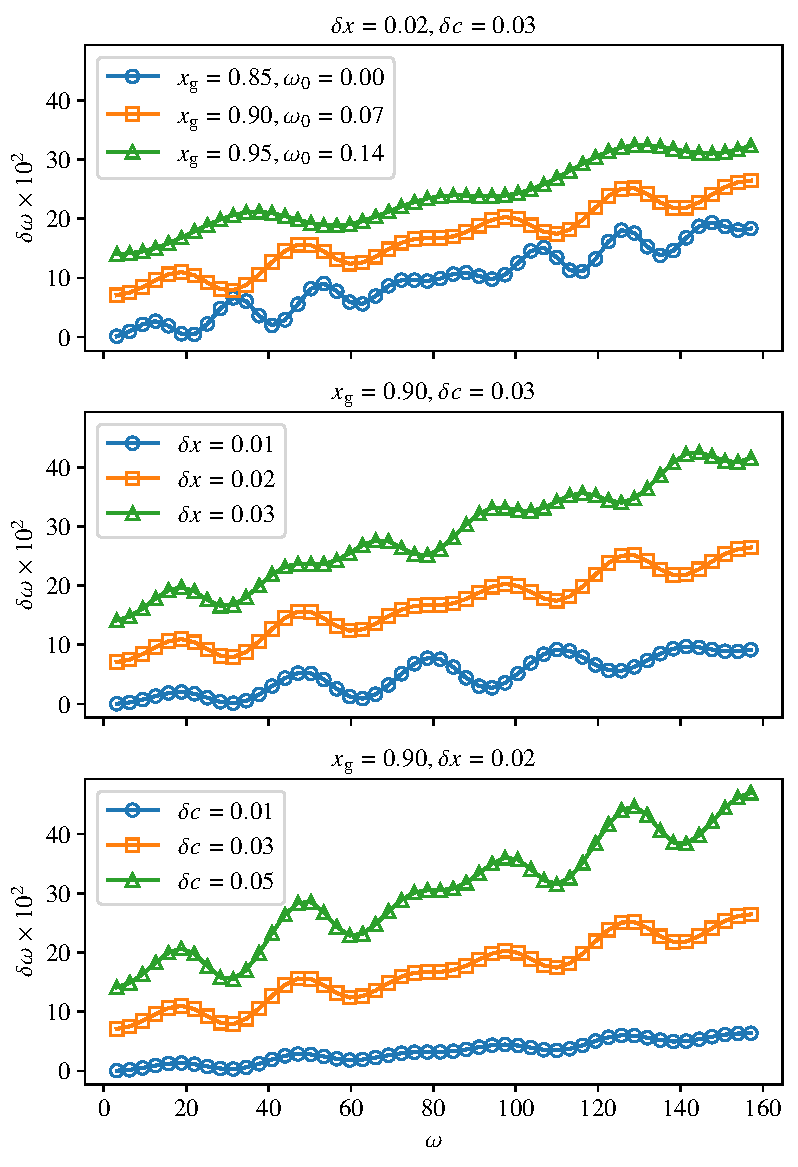
\includegraphics{figures/glitch-1d-example-results.pdf}
    \caption[The change in mode frequency induced by a rapid change in sound speed for the 1D example.]{The change in mode frequency induced by a change in sound speed of \(\delta c\) from \(x_\glitch - \delta x\) to \(x_\glitch + \delta x\) in a one-dimensional medium, bound such that \(x \in [0, 1]\) (see Figure \ref{fig:1d-diagram}). Outside the perturbation the speed of sound, \(c=1\). The frequency perturbations are offset by \(\omega_0\) given in the legend of the top panel. Points are joined by straight lines to guide the eye but do not represent real solutions.
    }
    \label{fig:1d-results}
\end{figure}

Let us use \(\omega'_n\) to denote the solutions to Equation \ref{eq:1d-glitch-sol}, where \(n\) is a positive integer. We find \(\omega'_n\) by solving Equation \ref{eq:1d-glitch-sol} using Newton's method for \(n = 1,\dots,50\) modes. Using dimensionless units of length and time, we set \(c=1\), \(L=1\), and test several values of \(x_\glitch\), \(\delta x\), and \(\delta c\). Initial guesses for \(\omega'_n\) are obtained from the homogeneous medium solutions (\(\omega_n\)) in Equation \ref{eq:omega-n}. We show the difference between the glitch solutions and those from the homogeneous medium, \(\delta \omega_n = \omega'_n - \omega_n\), in Figure \ref{fig:1d-results}. We can see a periodic component to \(\delta\omega\) induced by the glitch. As the wave nodes pass in and out of the region with changing \(n\), the sensitivity of the wave to the glitch varies periodically. The overall sensitivity to the glitch depends on how much the wave changes inside the glitch, hence why low \(n\) modes have smaller \(\delta\omega\).

% Physically, this arises from the change in phase required to satisfy the boundary conditions of the glitch region.

The functional form of \(\delta\omega\) appears to have a linear component and a short periodicity modulated by a longer periodicity. As the location of the glitch (\(x_\glitch\)) gets smaller, the short period of \(\delta\omega\) decreases. If we imagine the spacial distribution of nodes in the system as a function of \(n\), the density of nodes is larger towards the centre of the system. The periodicity arises from the nodes passing in and out of the glitch region with changing \(n\). Therefore, where the density of wave nodes is higher, we expect the short period of \(\delta\omega\) to decrease. Similarly, as the half-width of the glitch (\(\delta x\)) increases, the longer period increases. 

Furthermore, an increasing change in sound speed (\(\delta c\)) increases the amplitude of \(\delta\omega\). This result is intuitive, as we expect a larger change in \(c\) to correspond to a large change in \(\omega\). Finally, increasing both \(\delta x\) and \(\delta c\) increases the slope of \(\delta\omega\). The sensitivity of a mode to the glitch increases with \(n\) and depends on how much the wave changes in the glitch region. Modes of smaller \(n\) become more sensitive to the glitch region as \(\delta x\) and \(\delta c\) increase, thus increasing the linear slope of \(\delta\omega\).

%This may be interpreted as the nodes of each standing wave passing in and out of region 2 with increasing \(n\). Where there is a node, the wave is least sensitive to a change in structure, and 

\begin{figure}
    \centering
    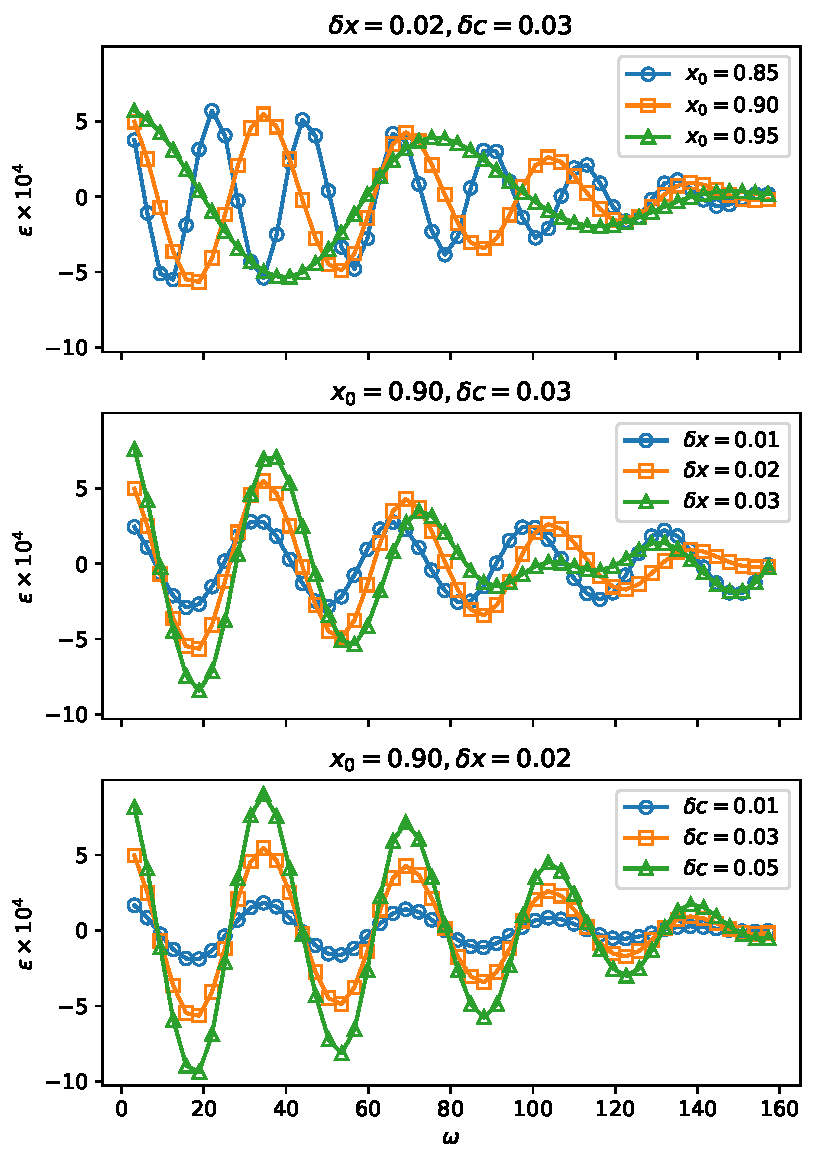
\includegraphics{figures/glitch-1d-example-phase.pdf}
    \caption[The same as Figure \ref{fig:1d-results} but showing the phase offset required to satisfy the boundary conditions.]{The same as Figure \ref{fig:1d-results} but showing the phase offset \(\epsilon\) required to satisfy the boundary conditions.}
    \label{fig:1d-phase}
\end{figure}

The small phase offset \(\epsilon\) in Equation \ref{eq:1d-phase} is required for the wave function to satisfy the boundary conditions at \(x = 0\). However, adding \(\epsilon\) shifts the effective location of \(x_\glitch\) --- it changes the scale of the \(x\)-axis by a factor of \((1 + \epsilon)\). We plot \(\epsilon\) against \(\omega\) in Figure \ref{fig:1d-phase} and show that its magnitude is \(\sim 10^{-4}\), much smaller than the location and size of region 2. The periodicity caused by the glitch also shows up in Figure \ref{fig:1d-phase}, with its properties affected similarly to Figure \ref{fig:1d-results}. This is because the more a mode is affected by the glitch, the greater the phase offset required to satisfy the boundary conditions.

Finding an approximate solution for \(\delta\omega\) is beyond the scope of this example. However, we can show that by modelling \(\delta\omega\), we can recover information about the structural glitch. Let us build a model \(\delta\omega = f(\omega)\). Looking at Figure \ref{fig:1d-results}, we propose a form for \(f\),
%
\begin{equation}
    f(\omega) = a_1 \omega - a_2 \sin (\tau_1 \omega) \cos (\tau_2 \omega), \label{eq:1d-domega-func}
\end{equation}
%
where \(a_1\) and \(a_2\) are coefficients which are both functions of \(\delta x\) and \(\delta c\). Parameters \(\tau_1\) and \(\tau_2\) are the `frequencies' (with dimensionless units of time\footnote{An angular frequency in angular frequency space has units of time.}) of the periodic component to \(\delta\omega\). Given Figure \ref{fig:1d-results}, we expect \(\tau_1\) and \(\tau_2\) to be related to \(\delta x\) and \(x_\glitch\) respectively.

\begin{figure}[tb]
    \centering
    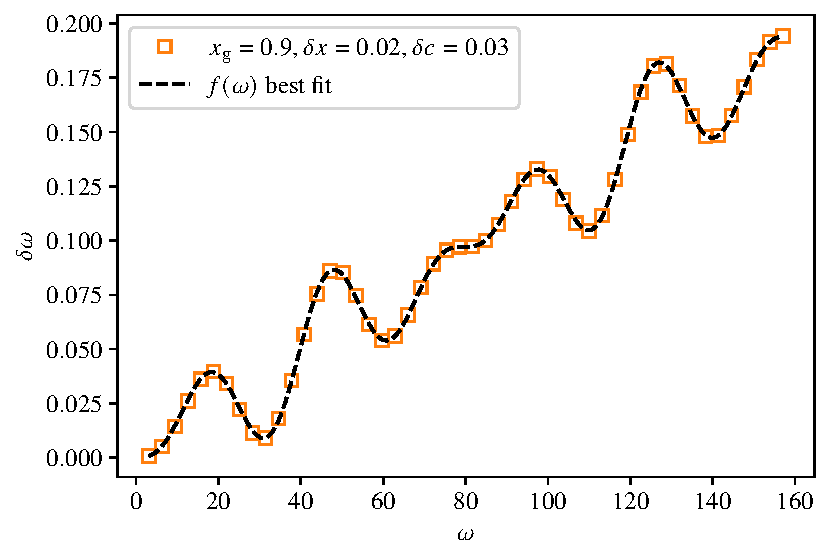
\includegraphics{figures/glitch-1d-fit.pdf}
    \caption{Best fit of Equation \ref{eq:1d-domega-func} to \(\delta\omega_n\) for \(n=1,\dots,50\), \(L=1\), and \(c=1\).}
    \label{fig:1d-fit}
\end{figure}

We fit Equation \ref{eq:1d-domega-func} to \(\delta\omega_n\) obtained from a glitch located at \(x_\glitch = 0.9\), with half-width \(\delta x = 0.02\), and change in sound speed \(\delta c = 0.03\). The best fitting line is shown in Figure \ref{fig:1d-fit}. We found \(\tau_1 \approx \num{0.0389}\) and \(\tau_2 \approx \num{0.199}\). The former corresponds to \(\tau_1 \simeq 2\delta\tau\), where \(\delta\tau\) is half the acoustic width of the glitch --- the time at which sound takes to transverse the region. Since the speed of sound \(c \approx \num{1}\) throughout the medium, the true value of \(\delta\tau \approx 0.02\). The latter `frequency' corresponds to \(\tau_2 \simeq 2\tau_\glitch\), where \(\tau_\glitch\) is the sound travel time from the nearest edge to the centre of the glitch (in this case \(\tau_\glitch \approx 0.1\)). Referring back to Figure \ref{fig:1d-results}, we can see how these relations should hold for different values of \(x_\glitch\), \(\delta x\), and \(\delta c\) providing the glitch region is small.

% NOTE: Could take this further to show a1 = 2 dc dtau / L and a2 = dc / L

It would be tempting to test this further, but we have shown that the glitch signature in \(\omega'_n\) relates to the properties of the glitch. Although the structure of a star is more complicated than this example, we can extend this principle to find glitch signatures in the mode frequencies of solar-like oscillators. Therefore, we will build upon this analogy in the next section where we review some examples of acoustic glitches in stars.

% NOTES: Go slowly through this. The next step is to fit a simple mode to theses oscillations and show that we can find x0 and dx. And show how the amplitude scales with dc.

% NOTES: When it comes to fitting the helium glitch, consider first fitting a GP to the modes with a free noise term. Fix the kernel scale to a series of values and show that we can see the glitch in the residuals. Of course, this leaves the question of what kernel scale to use. Well, we could just model everything at once!

\section[Acoustic Glitches in Stars]{Acoustic Glitch Signatures in Stellar Oscillations}\label{sec:glitch-star}

In the previous section, we considered a glitch in a homogeneous medium, where the speed of sound is constant everywhere else. In a star, the adiabatic sound speed is not constant. It depends on the density (\(\rho\)) and pressure (\(P\)),
%
\begin{equation}
    c^2 = \gamma \frac{P}{\rho},\label{eq:sound}
\end{equation}
%
where \(\gamma\) is the first adiabatic exponent,
%
\begin{equation}
    \gamma = \left( \frac{\partial \ln P}{\partial \ln \rho} \right)_S,
\end{equation}
%
at constant entropy, \(S\). \citet{Chandrasekhar1939} introduced three adiabatic exponents (\(\Gamma_1,\Gamma_2,\Gamma_3\)) to describe the non-ideal gas inside a star. However, in this chapter we do not use the other two and hence refer the first as \(\gamma \equiv \Gamma_1\).

For the most part, \(\gamma\), \(P\), and \(\rho\) change smoothly with radius inside a star. However, a rapid structural glitch in these quantities would lead to a sudden change in sound speed. In the previous section, we showed how such a perturbation can lead to a periodicity in the eigenfrequencies for a homogeneous medium. Characterising this signal allowed us to measure the properties of the glitch. If similar glitches were present in a star, then we might be able to do the same. In this section, we explore the origins of glitches inside a solar-like star. Then, we see what effect these have on the eigenfrequencies, a quantity we can measure through asteroseismology.

Firstly, let us consider the sound speed profile of a Sun-like star. Particularly, we want to see how the sound speed changes on the timescale of a pressure wave travelling through the star. As discovered in Section \ref{sec:1d-glitch}, a convenient timescale to work with is the acoustic depth, \(\tau\). This is not to be confused with the symbol for stellar age in Chapter \ref{chap:hmd}. Here, we define \(\tau\) as the time taken for a pressure wave to travel from the surface (\(R\)) to some radius (\(r\)) in a star under the assumption of spherical symmetry,
%
\begin{equation}
    \tau(r) = \tau_0 - \int_0^{r} \frac{\dd r'}{c(r')},\label{eq:tau}
\end{equation}
%
where \(\tau_0\) is the acoustic radius of the star. We recall from Section \ref{sec:seismo} that \(\nu_0 \equiv (2\tau_0)^{-1}\) may be approximated by the large frequency separation (\(\Delta\nu_{nl}\)) in the asymptotic limit that \(l/n \rightarrow 0\).

\begin{figure}[tb]
    \centering
    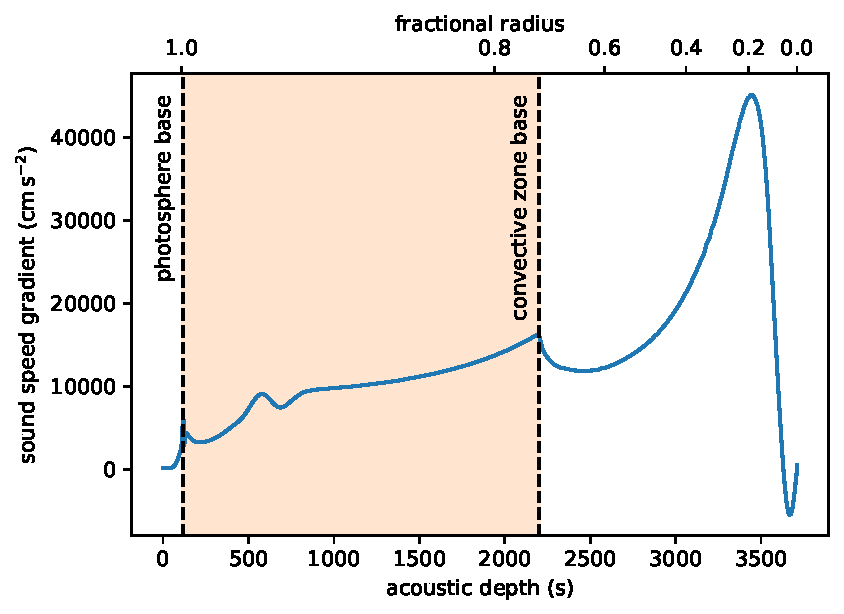
\includegraphics{figures/sound-speed-gradient.pdf}
    \caption[The sound speed gradient of model S plot against the acoustic depth.]{The sound speed gradient (\(\dd c/\dd \tau\)) of model S plot against the acoustic depth (\(\tau\)). The fractional radius to the photosphere base is given on the top axis. The convective envelope is shaded and the bases of the photosphere and convective zone are marked with dashed lines.}
    \label{fig:sound-speed-gradient}
\end{figure}

In Figure \ref{fig:sound-speed-gradient}, we show the sound speed gradient with respect to \(\tau\) for a Sun-like stellar model (model S; see Section \ref{sec:model-s}). We see how the speed of sound changes smoothly throughout the star. In the convective zone, there is a noticeable wiggle around \SI{700}{\second} and a sharp change in direction at its base. The first is caused by the ionisation of helium, which we will explore further in Section \ref{sec:helium-glitch}. The second is due to a discontinuity in the temperature gradient as the stellar interior goes from unstable due to convection to radiative. This will be discussed in Section \ref{sec:bcz-glitch}.

\subsection{Sun-Like Model Star}\label{sec:model-s}

We computed a representative Sun-like model star (hereafter `model S') using MESA \citep[version 12115;][]{Paxton.Bildsten.ea2011,Paxton.Cantiello.ea2013,Paxton.Marchant.ea2015,Paxton.Schwab.ea2018,Paxton.Smolec.ea2019,Jermyn.Bauer.ea2023}. The model was computed with a mass of \SI{1.0}{\solarmass} to a central fractional hydrogen abundance of \(X_c=0.6\). We used initial fractional helium and heavy-element abundances of \(Y_\mathrm{init} = 0.28\) and \(Z_\mathrm{init}=0.02\) respectively. The mixing-length was parametrised by \(\alpha_\mlt=1.9\) and a turbulent pressure factor of 1. We evolved the star using element diffusion with MESA's default coefficients \citep{Stanton.Murillo2016}. In addition, we used MESA's default \citet{Grevesse.Sauval1998} solar chemical composition and opacity tables. We also output pulsation profile data in FGONG format to later use when computing oscillation modes in Chapter \ref{chap:glitch-gp}. Our resulting model S had an age of \SI{4.073}{\giga\year}, \(\teff \approx \SI{5682}{\kelvin}\), and \(R \approx \SI{1.014}{\solarradius}\). Since the model was evolved with element diffusion, the surface fractional helium and heavy-element were approximately \(Y_\mathrm{surf} \approx 0.2515\) and \(Z_\mathrm{surf} \approx 0.01810\) respectively.

\subsection{Helium Ionisation Glitch}\label{sec:helium-glitch}

In this section, we will first show how the sound speed inside a solar-like star is affected by the ionisation of hydrogen and helium. Then, we will see that an increase in helium abundance (\(Y\)) increases the effect of helium ionisation on the speed of sound. Starting with the variational principle, we derive the frequently used equation for the glitch signature \(\delta\nu\) induced by the second ionisation of helium from \citet{Houdek.Gough2007}.

In the outer convective envelope of Sun-like stars, the temperature (\(\SIrange{e4}{e5}{\kelvin}\)) and density (\(\SIrange{e-5}{e-3}{\gram\per\centi\metre\cubed}\)) is suitable for ionising hydrogen and helium \citep{Eggleton.Faulkner.ea1973}. As a given chemical species in the star ionises, the number of particles and hence chemical potential of the species changes. This induces a gradient in the thermal free energy of the gas which relates to the pressure and entropy of the gas. Thus, we expect ionisation to cause a change in the pressure-density gradient at constant entropy, \(\gamma\). Since \(\gamma\) relates to the sound speed from Equation \ref{eq:sound}, any sudden change in \(\gamma\) will induce a change in \(c\).

\begin{figure}[tb]
    \centering
    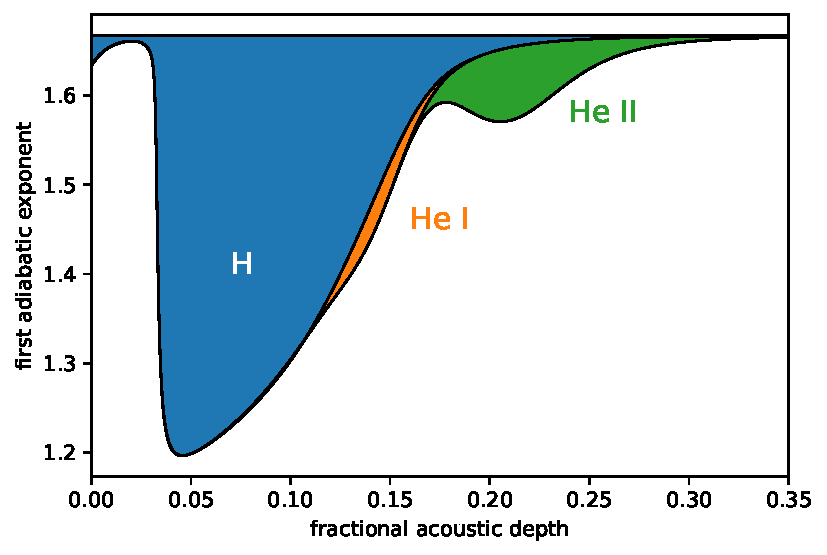
\includegraphics{figures/adiabatic-ionisation-regions.pdf}
    \caption[The depressions in the first adiabatic exponent caused by the ionisation of hydrogen and helium.]{The depressions in the first adiabatic exponent (\(\gamma\)) caused by the ionisation of hydrogen (H), and the first and second ionisations of helium (He\,\textsc{i} and He\,\textsc{ii}). The horizontal axis is the fractional acoustic depth from the surface of the star, \(\tau/\tau_0\).}
    \label{fig:gamma-zones}
\end{figure}

In Figure \ref{fig:gamma-zones}, we show \(\gamma\) for model S against fractional acoustic depth, shaded by regions of ionisation. For an ideal monatomic gas, \(\gamma=5/3\), but we see that \(\gamma < 5/3\) in regions where helium and hydrogen ionise. Close to the surface of the star, hydrogen ionisation has the largest effect on \(\gamma\) because it makes up the majority of stellar matter. The first (He\,\textsc{i}) and second (He\,\textsc{ii}) ionisations of helium occur deeper in the star. We can see that the second ionisation of helium has a greater effect on \(\gamma\) than the first. The effect of the He\,\textsc{ii} ionisation causes a rapid change in \(\gamma\) over a few per cent in \(\tau\) (equivalent to \(\sim \SI{100}{\second}\) in model S).

\subsubsection{The Effect of Helium Abundance on \(\gamma\)}

\begin{figure}
    \centering
    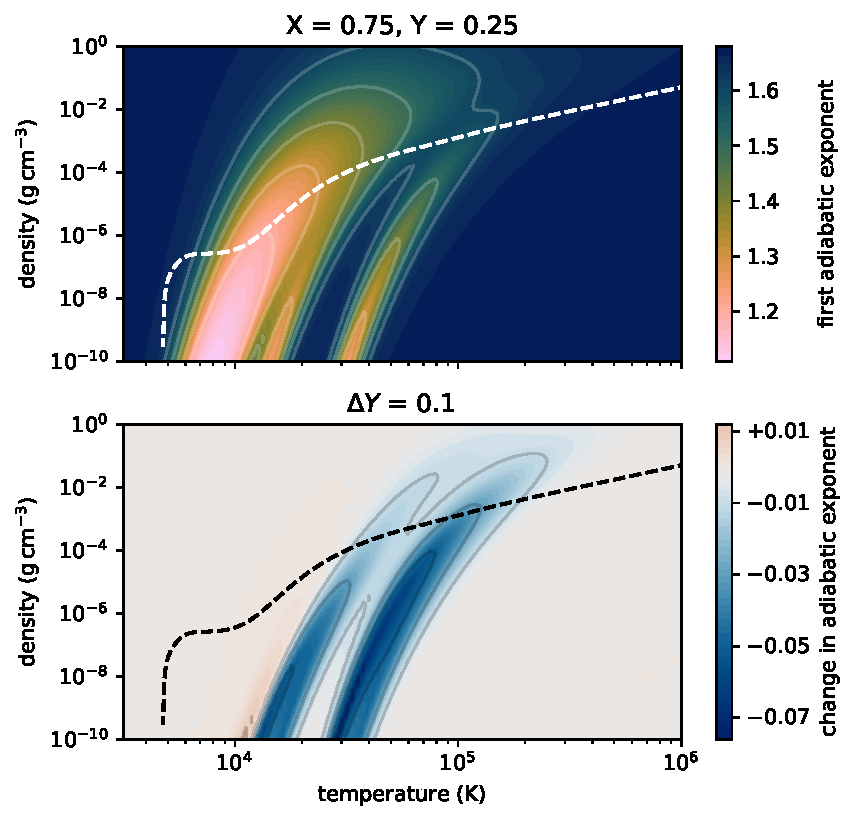
\includegraphics{figures/adiabatic-ionisation-temp.pdf}
    \caption[Temperature-density profile for a Sun-like star.]{Temperature-density profile for a Sun-like star. \emph{Top:} The first adiabatic exponent \(\gamma\) as a function of temperature and density, calculated using Eq. 53 of \citet{Houdayer.Reese.ea2021} for a helium mass fraction, \(Y=0.25\). \emph{Bottom:} The change in \(\gamma\) induced by a change in helium abundance, \(\Delta Y = 0.1\). In both panels, the dashed line shows the temperature-density profile of model S. \emph{This figure is a recreation of Fig. 5 in \citet{Houdayer.Reese.ea2021}.}}
    \label{fig:gamma-temp-density}
\end{figure}

We were able to isolate the contributions to \(\gamma\) from ionisation using a recent derivation by \citet{Houdayer.Reese.ea2021}. They obtained an approximate formula for \(\gamma\) as a function of temperature (\(T\)) and density valid for the outer convective zone of Sun-like stars. Using their formula, we plot \(\gamma\) for a range of \(T\) and \(\rho\) in Figure \ref{fig:gamma-temp-density}. The first panel illustrates the three ionisation regions of hydrogen and helium. The value of \(\gamma\) decreases when the ionisation reaction is occurring. The magnitude of this effect depends on the intersection with the temperature-density profile of the star (over-plot for model S). We can imagine a hotter star shifting this line such that ionisation occurs closer to the surface. Along the model S profile, we see that an increase in helium abundance by 0.1 decreases \(\gamma\) by up to \(\sim 0.03\) in the He\,\textsc{ii} ionisation region. This shows that helium abundance correlates with the depth of the glitch in \(\gamma\). However, there is clearly still some dependence on \(T\) and \(\rho\) which are governed by mass, chemical composition, and evolutionary phase.

% The exact effect of ionisation on \(\gamma\) is not known analytically. However, \citet{Houdayer.Reese.ea2021} recently approximated \(\gamma\) for the convective zone of a Sun-like star in their study of the helium ionisation glitch. In this subsection, we combine the equations derived in their work to help us understand the relation between ionisation and \(\gamma\). Let us consider an \(M\) mass star with fractional hydrogen and helium abundances of \(X\) and \(Y\) respectively. From \citet{Houdayer.Reese.ea2021}, we approximate the first adiabatic exponent as,
% %
% \begin{equation}
%     \gamma \simeq \frac{5}{3} - \frac{2}{3} \, \eta(T, \rho), \label{eq:gamma1}
% \end{equation}
% %
% where \(\eta\) represents the depression in \(\gamma\). Considering a hydrogen-helium mixture where \(X + Y \approx 1\), \(\eta\) is,
% %
% \begin{equation}
%     \begin{split}
%         \eta(T, \rho) &= \frac{1}{\partial_{TT}^2 f} \left[n_\hydrogen y_\hydrogen \, (1 - y_\hydrogen) \, \frac{(\chi_\hydrogen / k_B T)^2}{2 - y_\hydrogen}
%         % \right. \\ &\left. 
%         + n_\helium y_\helium^{(1)} \left(1 - y_\helium^{(1)}\right) \left(\frac{\chi_\helium^{(1)}}{k_B T}\right)^2 
%         \right. \\ &\left.
%         + \, n_\helium y_\helium^{(2)} \left(1 - y_\helium^{(2)}\right) \left(\frac{\chi_\helium^{(2)}}{k_B T}\right)^2\right],
%     \end{split}
% \end{equation}
% %
% where \(k_B\) is the Boltzmann constant. The parameter \(\partial_{TT}^2\) is the second partial derivative of the free energy density with respect to temperature (\(T\)),
% %
% \begin{equation}
%     \begin{split}
%         \partial_{TT}^2 f &\simeq \frac{3}{2} + n_\hydrogen y_\hydrogen \left[ \frac{3}{2} + \frac{(1 - y_\hydrogen)}{2 - y_\hydrogen} \left(\frac{3}{2} + \frac{\chi_\hydrogen}{k_B T}\right)^2 \right] %\\
%         + n_\helium y_\helium^{(1)} \left[ \frac{3}{2} + \left(1 - y_\helium^{(1)}\right) \left(\frac{3}{2} + \frac{\chi_\helium^{(1)}}{k_B T}\right)^2 \right] \\
%         &+ n_\helium y_\helium^{(2)} \left[ \frac{3}{2} + \left(1 - y_\helium^{(2)}\right) \left(\frac{3}{2} + \frac{\chi_\helium^{(2)}}{k_B T}\right)^2 \right],
%     \end{split}
% \end{equation}
% %
% where \(n_\mathbb{X} = N_\mathbb{X} / N\) is the number density and \(\chi_\mathbb{X}^{i}\) is the \(i\)-th ionisation energy of species \(\mathbb{X}\). Parameter \(y_\mathbb{X}^i\) is related to a reduced form of Saha's equation \needcite,
% %
% \begin{equation}
%     \frac{(y_\mathbb{X}^i)^q}{1 - y_\mathbb{X}^i} = \frac{2 g_\mathbb{X}^i}{g_\mathbb{X}^{i-1}} \frac{\overline{m}}{\rho \lambda_\ee^3} \, \ee^{- \chi_\mathbb{X}^i / k_B T},
% \end{equation}
% %
% where \(q = 2\) for hydrogen, \(q = 1\) for helium, \(\overline{m} = M/N\) is the mean mass, and \(g_\mathbb{X}^i\) is the ground-state degeneracy of ionisation state \(i\). We used these equations to produce Figures \ref{fig:gamma-zones} and \ref{fig:gamma-temp-density}.

\begin{figure}
    \centering
    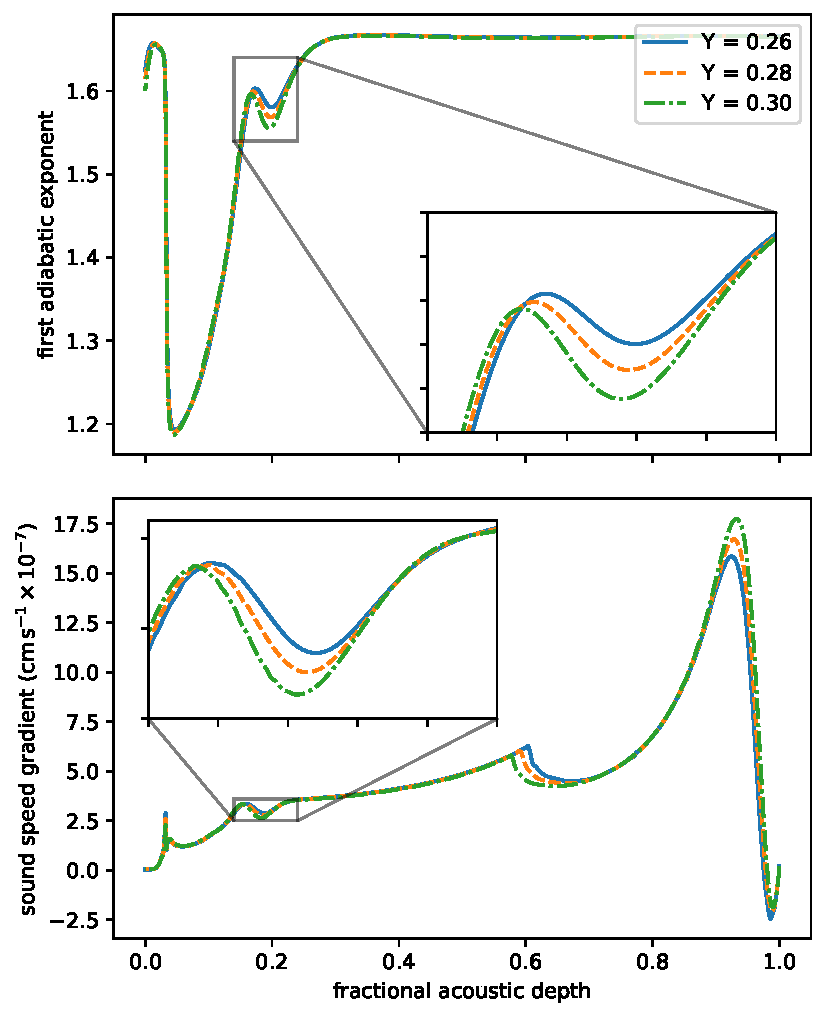
\includegraphics{figures/helium-ionisation-sound-speed.pdf}
    \caption[The effect on the sound speed profile for three solar-like stars with initial helium mass fractions of 0.26, 0.28, and 0.3.]{The effect on the sound speed profile for three solar-like stars with initial helium mass fractions of 0.26 (\emph{solid}), 0.28 (\emph{dashed}), and 0.3 (\emph{dot-dashed}). The models were each evolved to a central helium mass fraction of 0.6. \emph{Top:} The first adiabatic exponent \(\gamma\). \emph{Bottom:} The sound speed gradient \(\dd c/\dd t\) where \(t = \tau/\tau_0\) is the fractional acoustic depth.}
    \label{fig:gamma-sound-speed}
\end{figure}

To show the effect of small changes in \(Y\) on the sound speed, we plot the sound speed gradient in Figure \ref{fig:gamma-sound-speed}. The three models shown were evolved to the same \(X_c = 0.6\) as model S with initial helium abundances of 0.26, 0.28, and, 0.3. The dominant effect of helium abundance appears as a Gaussian-like depression in \(\gamma\) around the second ionisation of helium. We see how larger helium abundance increases the width and depression in \(\gamma\), which is reflected in the sound speed gradient. A larger \(Y\) also leads to a relative reduction in hydrogen abundance (\(X\)) which shrinks the width of the hydrogen ionisation region.

\subsubsection{The Effect of a Change in \(\gamma\) on p Mode Frequencies}

To see how a change in \(\gamma\) affects the mode frequencies, we explore the sensitivity of a mode to rapid structural changes in the star. Starting with the variational principle, we can approximate the characteristic frequencies of a spherically symmetric, slowly rotating star by \citep{Chandrasekhar1964},
%
\begin{equation}
    \omega^2 = \frac{\mathcal{E}}{\mathcal{I}}\label{eq:var-prin}
\end{equation}
%
which is a ratio of \(\mathcal{E}\) (proportional to the mode's energy)
%
% \begin{equation}
%     \mathcal{E} = \int_0^R \left[\gamma P (\dive{\vect{\xi}})^2 + 2(\vect{\xi}\cdot \nabla P) \dive{\vect{\xi}} + (\vect{\xi}\cdot \nabla P) (\vect{\xi}\cdot\nabla\ln\rho)\right] r^2 \, \dd r.
% \end{equation}
%
to its inertia (\(\mathcal{I}\)). The mode inertia is given by,
%
\begin{equation}
    \mathcal{I} = \int_0^R \vect{\xi} \cdot \vect{\xi} \, \rho r^2 \, \dd r,
\end{equation}
%
where the amplitude and direction of a pressure wave at a given point in a star is given by the so-called Lagrangian perturbation vector \(\vect{\xi}\). 

\begin{figure}
    \centering
    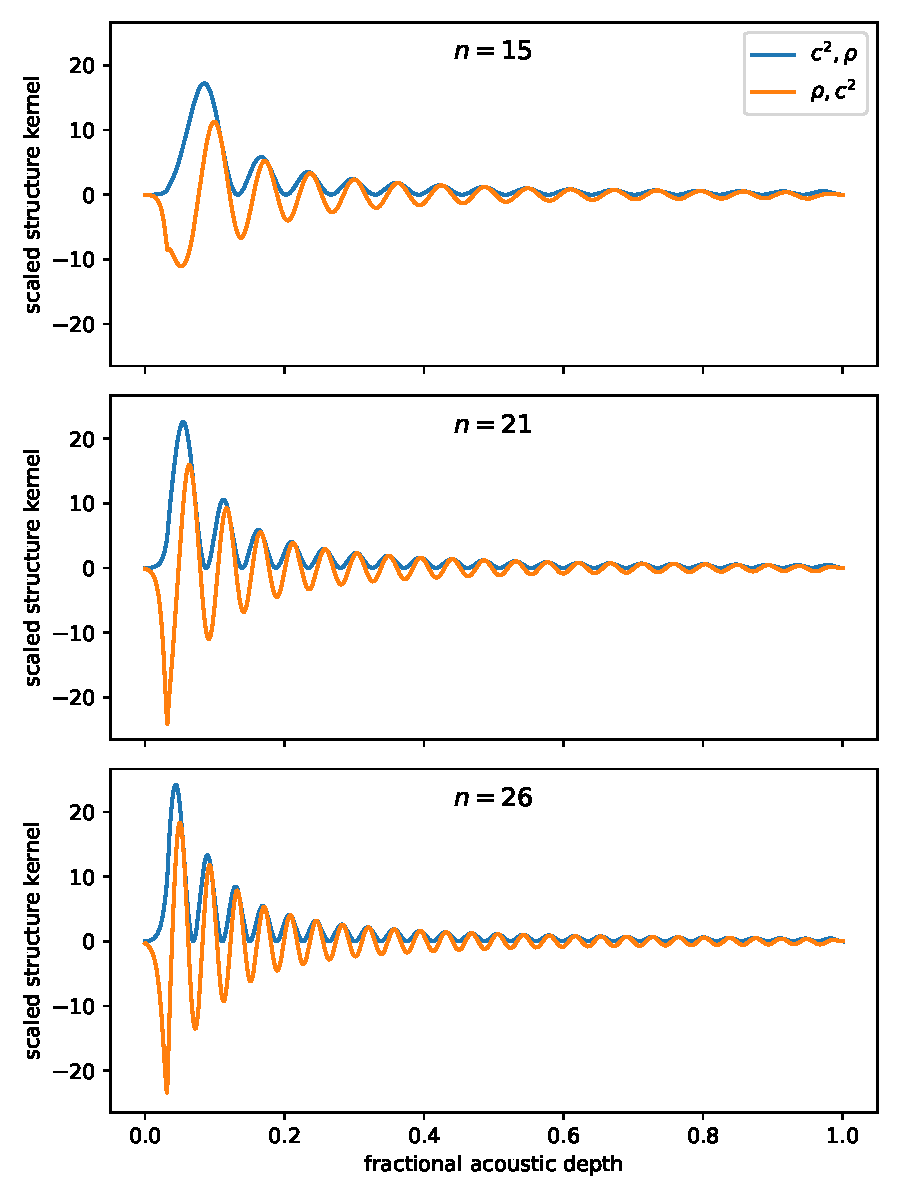
\includegraphics{figures/kernels.pdf}
    \caption[Structure kernels (\(\mathcal{K}_{c^2,\rho}, \mathcal{K}_{\rho,c^2}\)) scaled by the stellar radius as a function of fractional acoustic depth.]{Structure kernels (\(\mathcal{K}_{c^2,\rho}, \mathcal{K}_{\rho,c^2}\)) scaled by the stellar radius as a function of fractional acoustic depth. The kernels were computed for three radial oscillation modes (\(n=15,21,26\)) using oscillation calculations for stellar model S.}
    \label{fig:kernels}
\end{figure}

A structural glitch in the star would cause a small change in frequency (\(\delta\omega\)). Differentiating both sides of Equation \ref{eq:var-prin} with respect to \(\omega\), we get,
%
\begin{align}
    2\omega &= \frac{1}{\mathcal{I}} \left( \frac{\delta\mathcal{E}}{\delta\omega} - \omega^2 \frac{\delta\mathcal{I}}{\delta\omega}\right), \qquad \left[\times \frac{\delta\omega}{2\omega^2}\right] \notag \\
    \frac{\delta\omega}{\omega} &= \frac{1}{2\,\mathcal{I}} \left(\frac{\delta\mathcal{E}}{\omega^2} - \delta\mathcal{I}\right).
\end{align}
%
Small changes \(\delta\mathcal{E}\) and \(\delta\mathcal{I}\) depend on changes to the state variables. By perturbing and substituting appropriate forms of \(\mathcal{E}\) and \(\mathcal{I}\), it is possible to rewrite this as a function of the so-called structural kernels \(\mathcal{K}_{a,b}\). For example \citep{Christensen-Dalsgaard2014},
%
\begin{equation}
    \frac{\delta\omega}{\omega} = \int_0^R \left(\mathcal{K}_{c^2,\rho} \frac{\delta c^2}{c^2} + \mathcal{K}_{\rho,c^2} \frac{\delta \rho}{\rho} \right) \dd r.\label{eq:kernels}
\end{equation}
%
where \(\mathcal{K}_{a, b}\) gives the relative effect on \(\omega\) at a given \(r\) due to a perturbation in a state variable \(a\) at fixed \(b\). The kernels, defined fully in \citet{Gough.Thompson1991}, can show the sensitivity of the wave to a change in state in the star. We plot \(\mathcal{K}_{c^2,\rho}\) and \(\mathcal{K}_{\rho,c^2}\) in Figure \ref{fig:kernels} for a few radial oscillation modes. Both decay through the star, meaning that the modes are less sensitive to structural changes deeper in the star. The kernels also oscillate at different frequencies corresponding to the radial order, meaning the amount they intersect with a glitch changes with \(\omega\).

We can evaluate Equation \ref{eq:kernels} to find the effect on \(\omega\) due to a change in \(\gamma\) from helium ionisation. The first term can be easily rewritten in terms of a change in \(\gamma\) because \(c^2 \propto \gamma\), hence \(\mathcal{K}_{\gamma,\rho} \delta \gamma / \gamma \equiv \mathcal{K}_{c^2,\rho} \delta c^2 / c^2\). Helium ionisation has a negligible effect on density, so we can assume \(\delta\rho/\rho \approx 0\) in the ionisation region. Therefore, we may rewrite Equation \ref{eq:kernels} due to a change in \(\gamma\) as,
%
\begin{equation}
    \left.\frac{\delta\omega}{\omega}\right|_\gamma \simeq \int_0^R \mathcal{K}_{\gamma,\rho} \frac{\delta\gamma}{\gamma} \dd r,\label{eq:delta-omega}
\end{equation}
%
where \(\mathcal{K}_{\gamma,\rho}\) is shown in \citet{Gough1993} to satisfy,
%
\begin{equation}
    \omega^2 \mathcal{I}\mathcal{K}_{\gamma,\rho} = \frac12 \gamma P (\dive{\vect{\xi}})^2 r^2.\label{eq:gamma-kernel}
\end{equation}
%

\newcommand*{\propconst}{\ensuremath{{\mathcal{A}}}}

In order to solve Equation \ref{eq:delta-omega}, we first expand the mode inertia, \(\mathcal{I}\). The Lagrangian perturbation vector can be written in terms of a radial and horizontal component, \(\vect{\xi} = \xi_r \hat{r} + \vect{\xi}_h\). In the high-order limit where \(l/n \rightarrow 0\), the horizontal component \(\vect{\xi}_h\) is negligible. Therefore, we can rewrite the mode inertia as,
%
\begin{equation}
    \mathcal{I} \simeq \int_0^R \xi_r^2 \rho r^2 \, \dd r.
\end{equation}
%
Then, we use a suitable approximation of \(\xi_r\) from \citet{Gough1993}, 
%
\begin{equation}
    \xi_r \simeq \frac{\propconst}{r}\sqrt{\frac{K}{\rho}} \cos\psi,\label{eq:xi-r}
\end{equation}
%
where \(\propconst\) is a proportionality constant. The radial wave number \(K \simeq \omega / c\) for high-order acoustic modes. 
% Because the speed of sound changes slowly between nodes?
Assuming \(\tau\) is not close to the upper turning point (where the wave is reflected near the stellar surface), the phase term \(\psi \simeq \omega \tau + \epsilon\). The small offset \(\epsilon\) is a slowly varying function of \(\tau\). Substituting Equation \ref{eq:xi-r} into the mode inertia gives,
%
\begin{align}
    \mathcal{I} &\simeq \propconst^2 \int_0^R K \cos^2\psi \, \dd r, \notag \\
    &= \frac12 \omega \propconst^2 \int_0^R (1 + \cos 2 \psi) \frac{\dd r}{c}.
\end{align}
%
Finally, changing to an integral over the acoustic depth, \(\tau\) we can evaluate the integral for high-order modes where \(\omega_n \ll \tau_0^{\,-1}\),
%
\begin{equation}
    \mathcal{I} \simeq \frac12 \omega \propconst^2 \int_0^{\tau_0} [1 + \cos 2 (\omega\tau + \epsilon)] \, \dd \tau \simeq \frac12 \omega \propconst^2 \tau_0. \label{eq:inertia}
\end{equation}
%

Secondly, we substitute an approximation for \((\dive{\vect{\xi}})^2\) from \citet{Gough1993},
%
\begin{equation}
    (\dive{\vect{\xi}})^2 \simeq \frac{\propconst^2 \omega^3}{\gamma P c r^2} \sin^2\psi, \label{eq:div-xi}
\end{equation}
%
into Equation \ref{eq:gamma-kernel} to get,
%
\begin{align}
    \left.\frac{\delta\omega}{\omega}\right|_\gamma &\simeq \frac{1}{2\omega^2\mathcal{I}} \int_0^{R} \delta\gamma P (\dive{\vect{\xi}})^2 r^2 \, \dd r, \notag \\
    &\simeq \frac{\omega \propconst^2}{2 \mathcal{I}} \int_0^{R} \frac{\delta\gamma}{\gamma}\sin^2\psi\frac{\dd r}{c}, \notag \\
    &= \frac{\omega \propconst^2}{4 \mathcal{I}} \int_0^{R} \frac{\delta\gamma}{\gamma}(1 - \cos 2\psi)\frac{\dd r}{c}.
\end{align}
%
We can see that \(\delta\omega\) is split into a smooth and a periodic component. The smooth component may be treated later, but for now we focus on the oscillating part of \(\delta\omega\). Substituting \(\mathcal{I}\) from Equation \ref{eq:inertia} and changing to an integral over acoustic depth we get,
%
\begin{equation}
    \left.\frac{\delta\omega}{\omega}\right|_{\gamma,\mathrm{osc}} \simeq - \frac{1}{2\tau_0} \int_0^{\tau_0} \frac{\delta\gamma}{\gamma} \cos 2 (\omega\tau + \epsilon) \, \dd \tau. \label{eq:omega-osc}
\end{equation}
%

\subsubsection{A Functional Form of the Helium Glitch Signature}

We have shown that a change in \(\gamma\) can induce a periodicity in \(\omega\). The functional from of this periodicity depends on \(\delta\gamma/\gamma\). As shown in Figures \ref{fig:gamma-zones} and \ref{fig:gamma-temp-density}, the dominant change in \(\gamma\) due to a change in helium abundance is from the second ionisation of helium. There have been different attempts to approximate \(\delta\gamma/\gamma\,|_\heII\) in the literature, for example using a Dirac delta function or a triangular function \citep{Monteiro.Christensen-Dalsgaard.ea1994,Monteiro.Thompson2005}. In recent years, work modelling the glitch has used the formulation from \citet{Houdek.Gough2007} where the change in \(\gamma\) due to He\,\textsc{ii} ionisation is modelled with a Gaussian shape,
%
\begin{equation}
    \left.\frac{\delta\gamma}{\gamma}\right|_\heII \simeq - \frac{\Gamma_\heII}{\Delta_\heII \sqrt{2\pi}} \, \ee^{- \frac12{(\tau - \tau_\heII)^2}/{\Delta_\heII^2} }, \label{eq:he-gamma}
\end{equation}
%
where \(\Gamma_\heII\) is the area, \(\Delta_\heII\) is the characteristic width, and \(\tau_\heII\) is the centre of the ionisation region.

Here, we verify the result for \(\delta\omega\) due to He\,\textsc{ii} ionisation from \citet{Houdek.Gough2007}. Substituting Equation \ref{eq:he-gamma} into Equation \ref{eq:omega-osc} with a change of variables to \(x = (\tau - \tau_\heII)/\Delta_\heII\), we get,
%
\begin{equation}
    \left.\frac{\delta\omega}{\omega}\right|_{\heII, \mathrm{osc}} \simeq \frac{\Gamma_\heII}{2\sqrt{2\pi} \, \tau_0} \, \int_{-\infty}^\infty \ee^{- x^2/2} \cos 2 (\Delta_\heII \omega x + \widetilde{\epsilon_\heII}) \, \dd x \label{eq:omega-ii-osc}
\end{equation}
%
where \(\widetilde{\epsilon_\heII} = \omega\tau_\heII + \epsilon_\heII\) and the phase \(\epsilon=\epsilon_\heII\) is assumed constant across the glitch region. We can solve the above integral analytically using differentiation under the integral sign by introducing an arbitrary variable \(a\),
%
\begin{equation}
    I(a) = \int_{-\infty}^\infty \ee^{- x^2/2 } \cos 2 (\Delta_\heII \omega x a + \widetilde{\epsilon_\heII}) \, \dd x
\end{equation}
%
Differentiating this with respect to \(a\), and then integrating by parts gets,
%
\begin{align}
    I'(a) &= - 2 \Delta_\heII \omega \int_{-\infty}^\infty x \, \ee^{- x^2/2 } \sin 2 (\Delta_\heII \omega x a + \widetilde{\epsilon_\heII}) \, \dd x, \notag\\
    &= - 2 \Delta_\heII \omega \int_{-\infty}^\infty \sin 2 (\Delta_\heII \omega x a + \widetilde{\epsilon_\heII}) \, \dd \ee^{- x^2/2 }, \notag\\
    &= 2 \Delta_\heII \omega \left\{ \left[ \ee^{- x^2/2 } \sin 2 (\Delta_\heII \omega x a + \widetilde{\epsilon_\heII}) \right]_{-\infty}^\infty - 2 \Delta_\heII \omega a \int_{-\infty}^\infty \ee^{- x^2/2 } \cos 2 (\Delta_\heII \omega x a + \widetilde{\epsilon_\heII}) \, \dd x \right\}, \notag\\
    &= - 4 \Delta_\heII^2 \omega^2 a \, I(a),
\end{align}
%
which is a differential equation with the solution,
%
\begin{equation}
    \begin{split}
        I(a) = I(0) \ee^{- 2 \Delta_\heII^2 \omega^2 a^2}; \qquad I(0) &= \int_{-\infty}^\infty \ee^{- x^2/2 } \cos 2 \widetilde{\epsilon_\heII} \, \dd x, \\
        &= \sqrt{2\pi} \, \cos 2 \widetilde{\epsilon_\heII},
    \end{split}
\end{equation}
%
Therefore, if we set \(a = 1\) (to get back to the integral in Equation \ref{eq:omega-ii-osc}) we get the following for the periodic glitch signature \citep[cf.][Eq. 15]{Houdek.Gough2007},
%
\begin{equation}
    \left.\frac{\delta\omega}{\omega}\right|_{\heII, \mathrm{osc}} \simeq \frac{\Gamma_\heII}{2 \tau_0} \ee^{- 2 \Delta_\heII^2 \omega^2} \cos 2 (\tau_\heII\omega + \epsilon_\heII),
\end{equation}
%
We can rearrange this to a more familiar form in terms of cyclic frequency \citep[e.g.][]{Verma.Faria.ea2014,Verma.Raodeo.ea2017}, by substituting \(\omega = 2\pi\nu\),
%
\begin{equation}
    \left.\frac{\delta\nu}{\nu}\right|_{\heII, \mathrm{osc}} \simeq \nu_0 \Gamma_\heII \, \ee^{- 8 \pi^2 \Delta_\heII^2 \nu^2} \, \sin ( 4 \pi \tau_\heII \nu + \phi_\heII), \label{eq:he-osc}
\end{equation}
%
where \(\phi_\heII = 2(\epsilon_\heII + \pi/4)\), and \(\nu_0 = (2 \tau_0)^{-1}\) is the inverse acoustic diameter of the star.

\subsection{Base of the Convective Zone Glitch}\label{sec:bcz-glitch}

\begin{figure}[tb]
    \centering
    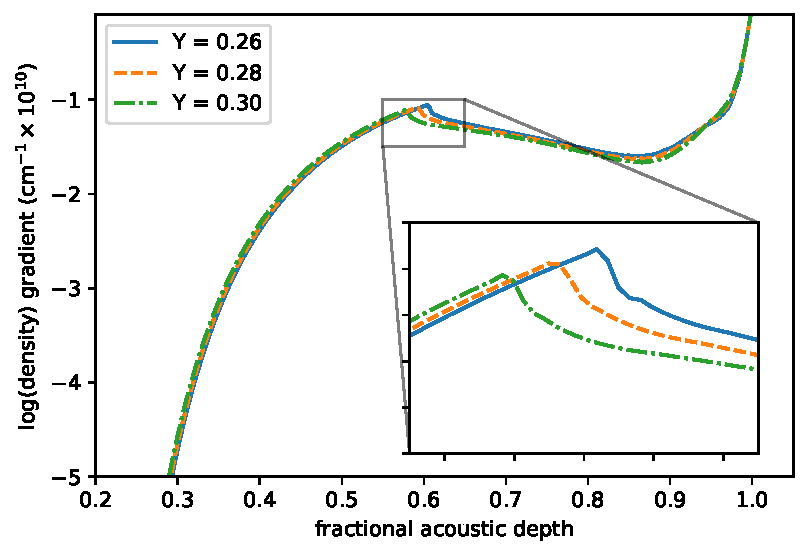
\includegraphics{figures/bcz-density-gradient.pdf}
    \caption[Discontinuity in the density gradient at the base of the convective zone for three solar-like model stars.]{Discontinuity in the density gradient at the base of the convective zone for three solar-like stars with initial helium mass fractions of 0.26 (\emph{solid}), 0.28 (\emph{dashed}), and 0.3 (\emph{dot-dashed}).}
    \label{fig:bcz-density}
\end{figure}

The sensitivity of p-modes to glitches gets smaller further into the star. However, we should not neglect the effect of the near-discontinuity at the base of the convective zone (BCZ). This arises from a jump in the second derivative of temperature at the BCZ which translated to discontinuities in the second derivative of density and sound speed. In Figure \ref{fig:bcz-density} we can see a fast change in direction of the density gradient around \(\tau/\tau_0 \approx 0.6\) (or at about \SI{2200}{\second} for model S). We also see that the relative location of the BCZ changes a little with \(Y\).

% Overshoot actually causes discontinuity in first derivative, not second \citep{Zahn1991}.

We could take a similar approach to the previous section, now considering the second kernel \(\mathcal{K}_{\rho,c^2}\) since the discontinuity affects \(\rho\). However, \citet{Houdek.Gough2007} take another approach by considering the discontinuity as it appears in the acoustic cut-off frequency, \(\omega_{ac}\). The details of this derivation are beyond the scope of this work. Instead, we quote their result for the change in frequency induced by the BCZ at an acoustic depth of \(\tau_\bcz\) \citep[cf.][Eq. 17]{Houdek.Gough2007},
%
\begin{equation}
    \left.\frac{\delta\omega}{\omega}\right|_{\bcz,\mathrm{osc}} \simeq \frac{c_\bcz^2\Delta_\bcz}{8\tau_0 \omega^3} \left(1 + {1}/{4\tau_0^2\omega^2}\right)^{-1/2} \cos\left[2(\tau_\bcz \omega + \epsilon_\bcz) + \tan^{-1}(2\tau_0\omega)\right]
\end{equation}
%
where \(\epsilon_\bcz\) is some phase which depends slowly on \(\omega\), \(c_\bcz\) is the speed of sound and,
%
\begin{equation}
    \Delta_\bcz = \left[\frac{\dd^2 \ln\rho}{\dd r^2}\right]_{-r_\bcz}^{+r_\bcz},
\end{equation}
%
is the change in second density derivative at the BCZ (\(r = r_\bcz\)).

For high-order modes, \(\tau_0 \omega \gg 1\) and thus \(\tan^{-1}(2\tau_0\omega) \simeq \pi/2\), and \((1 + {1}/{4\tau_0^2\omega^2})^{-1/2} \simeq 1\). Therefore, we can simplify this and write it in a more familiar form in terms of cyclic frequency,
%
\begin{equation}
    \left.\frac{\delta\nu}{\nu}\right|_{\bcz,\mathrm{osc}} \simeq \frac{c_\bcz^2\Delta_\bcz}{32\pi^3}\frac{\nu_0}{\nu^3} \sin(4\pi\tau_\bcz\nu + \phi_\bcz) \label{eq:bcz-osc}
\end{equation}
%
where \(\phi_\bcz\) is some approximately constant phase term.

Now we have equations for the effect of He\,\textsc{ii} ionisation and the BCZ for a given mode frequency \(\nu\), we can use them to model the glitch signatures as they appear in observed mode frequencies, \(\nu_{nl}\). Naturally, these equations are not exact. Several assumptions were made during their derivations. Therefore, if we want to model the glitch signature in \(\nu_{nl}\), we need some way of accounting for the uncertainty in the above equations. In the next chapter, we apply this model to characterise the glitch for some example stars. Although such models have been applied to other Sun-like stars before \citep[e.g.][]{Mazumdar.Monteiro.ea2014,Verma.Faria.ea2014}, we propose a new statistical model to account for the uncertainty in the functional form of \(\nu_{nl}\) with \(n\).
